\chapter{Implementation}
\label{ch:implementation}

In this chapter, we describe the implementation of the design we described in \Cref{ch:design}. You should \textbf{not} describe every line of code in your implementation. Instead, you should focus on the interesting aspects of the implementation: that is, the most challenging parts that would not be obvious to an average Computer Scientist. Include diagrams, short code snippets, etc. for illustration. 

\section{Data Collection}
To facilitate with the fine-tuning of the BERT/RoBERTa models and the training of the LSTM/RNN models,it was necessary to collect
a large amount of labelled data. As discussed in \ref{ch:background}, data was collected from Wikipedia and Reddit. Wikipedia was first
chosen due to the fact it has a large amount of data and all are labelled into categories. The one downside to Wikipedia is the style
of writing is very formal and factual which does not represent how social media posts are written. This is why Reddit was also used.
Reddit is a social media platform, whose subreddits give us a large amount of labelled data.\\
The input data went through a preprocessing step before being used to train the models.\\
A post/article corresponds to the input data, and the subreddit/wikipedia category corresponds to that inputs label. The data was collected
using the Reddit API and Wikipedia API.\\
After collecting all the data, there was roughly 1500 data points for each label (topic).
\subsection{Preprocessing}
Some preprocessing was necessary to clean the data. The proprocessing step would remove any punctuation and remove stopwords. This was done
to reduce the size of the input while keeping the most important words.\\
In retrospect, it could be possible that the self-attention mechanism of BERT/RoBERTa would be able to learn the context of some stopwords
and punctuation to improve the accuracy. This has been left as future work.
\subsection{Wikipedia Data}
Wikipedia data was colleceted using the Wikipedia API. There exists a python library called `Wikipedia-API' \cite{wikiapi} that acts as a wrapper
for the Wikipedia API. The library supplies useful functionalities such as:
\begin{itemize}
    \item \textbf{WikiAPI.page} - Takes in a string that acts as a query for the API. In this project the query string is ``Categroy:\{topic\}'' which returns a list of articles/subcategories
    \item \textbf{categorymembers.values()} - given the results of the page query, this function is used to return the articles/subcategories.
\end{itemize}
The way WikiAPI.page works means that we may be returned another category. Because of this, a recursive function is used to take the subcategories found and get
the articles from those subcategories. This could recurse on indefinitely, so a maximum depth of 1 was used to prevent this. A depth of 1 means that we get articles
from the main category and the subcategories of the main category. The recursive function fetches the titles of articles so they can be queried afterwards.
\begin{algorithm}
    \caption{$get\_category\_members$}\label{alg:cat-members}
\begin{algorithmic}
    \STATE $\text{\textbf{INPUT}: category, level, max\_level}$
    \STATE $category\_members \gets \text{list of articles in category}$
    \bindent
    \STATE $- \textbf{WikiAPI.page(``Category:\{category\}'').}\textbf{categorymembers.values()}}$
    \eindent
    \STATE $titles \gets \text{empty list}$
    \FOR{$\text{each member in category\_members}$}
        \IF{$\text{member is a category AND level<max\_level}$}
            \STATE $titles.append(get\_category\_members(member, level+1, max\_level))$
        \ELSE
            \STATE $titles.append(\text{title of member})$
        \ENDIF
    \ENDFOR
    \RETURN titles
\end{algorithmic}
\end{algorithm}

Using this function the labelled data can be collected as follows:
\begin{algorithm}
    \caption{$\text{Algorithm to Retrieve Wikipedia Data}$}\label{alg:wiki-data}
    \begin{algorithmic}
        \STATE $\text{topics} \gets \text{list of topics to collect data for}$
        \STATE $\text{data} \gets \text{empty list}$
        \FOR{$\text{each topic in topics}$}
            \STATE $titles \gets get\_category\_members(topic, 0, 1)$
            \FOR{$\text{each title in titles}$}
                \STATE $page \gets \text{WikiAPI.page(title)}$
                \STATE $text \gets \text{page.text}$
                \IF{$\text{text is empty}$}
                    \STATE $text \gets \text{page.summary}$
                \ENDIF
                \IF{$\text{text is empty}$}
                    \STATE $\text{\textbf{CONTINUE}}$
                \ENDIF
                \STATE $text \gets \text{preprocess(text)}$
                \STATE $data.append((page.content, topic))$
            \ENDFOR
        \ENDFOR
        \STATE $\text{Write fata to csv file}$
    \end{algorithmic}
\end{algorithm}

The algorithm loops through each topic and gets the article titles from `get\_category\_members`. It then loops through each title, attempts to find text in the page,
and if it does, it appends the preprocessed text and the topic to the data list. The data list is then written to a csv file.
\subsection{Reddit Data}
Reddit data was collected using the Reddit API. Their exists a python library called `PRAW` \cite{praw} that acts as a wrapper for the Reddit API.
The library provides useful functionalities. The ones used in this project are:
\begin{itemize}
    \item \textbf{PRAW.reddit} - Takes in API key and secret to authenticate with Reddit API. Returns a Reddit object that can be used to query the API.
    \item \textbf{reddit.subreddit} - Takes in a string that acts as a query for the API. In this project the query string is ``\{topic\}''.
    \item \textbf{subreddit.hot()} - Returns a list of hot posts in the subreddit. Optionally a limit parameter can be set.
\end{itemize}
These functions are used to get the data as follows:
\begin{algorithm}
    \begin{algorithmic}
        \STATE $\text{topics} \gets \text{list of topics to collect data for}$
        \STATE $\text{data} \gets \text{empty list}$
        \FOR{$\text{each topic in topics}$}
            \STATE $subreddit \gets \text{reddit.subreddit(topic)}$
            \STATE $hot \gets \text{subreddit.hot(limit=100)}$
            \FOR{$\text{each post in hot}$}
                \STATE $text \gets \text{preprocess(post.title + text)}$
                \STATE $data.append((text, topic))$
            \ENDFOR
        \ENDFOR
        \STATE $\text{Write fata to csv file}$
    \end{algorithmic}
\end{algorithm}
Fetching Reddit data is much simpler than fetching Wikipedia data due to the fact that when querying a subreddit, only posts are returned and no other subreddits.
\section{RNN and LSTM}
For creating the RNN and LSTM models, the `tensorflow' and `keras' libraries were used. This was to take advantage of the `tensorflow` GPU support on
the Department of Computer Science's (DCSs) batch compute system. Also, previous experience with these libraries made it easier to use them.\\
For both RNN and LSTM models the data was preprocessed in the same way. The data was tokenized using the `Keras Tokenizer` \cite{keras-tokenizer}. TODO:
what does a tokenizer do?
The output values were one-hot encoded using pandas `get\_dummies` \cite{pandas-dummies}. The data was split into training and testing sets using the `train\_test\_split`
function from `sklearn.model\_selection` \cite{sklearn-split}.\\
The RNN model was created using the `Sequentia' model from `keras'. A sequential model allows us to build up our model by adding layers. The architecture of the
model is as follows:
\begin{itemize}
    \item \textbf{Embedding} - TODO
    \item \textbf{Bidirectional(SimpleRNN)} - TODO
    \item \textbf{Dense} - TODO
    \item \textbf{Dense} - TODO
\end{itemize}
The model was compiled using the `categorical\_crossentropy` loss function and the `adam` optimizer. The model was trained for 10 epochs with a batch size of 64.\\
A bidirectional RNN was used to attempt to overcome the problem of unidirectionala context.\\\\
The LSTM model was created similarly to the RNN model. However, using a bidirectional LSTM instead of a bidirectional RNN. The architecture of the model is as follows:
\begin{itemize}
    \item \textbf{Embedding} - TODO
    \item \textbf{Bidirectional(LSTM)} - TODO
    \item \textbf{Dense} - TODO
    \item \textbf{Dense} - TODO
\end{itemize}
The same loss function and optimizer were used. The model was trained for 10 epochs with a batch size of 64.
\section{BERT}
To get the BERT model, the `tensorflow\_hub' library was used. This library gives developers access to pretrained models. The BERT model and preprocessing functions
can be imported as follows:
\begin{algorithm}
    \begin{algorithmic}
        \STATE preprocess = tensorflow\_hub.KerasLayer(``https://tfhub.dev/tensorflow/bert\_en\_uncased\_preprocess/3'')
        \STATE bert = tensorflow\_hub.KerasLayer(``https://tfhub.dev/tensorflow/small\_bert/bert\_en\_uncased\_L-4\_H-512\_A-8/1'')
    \end{algorithmic}
\end{algorithm}

When creating the model, these layers can be included in the model architecture. The architecture of the model is as follows:
\begin{itemize}
    \item \textbf{Input} - TODO
    \item \textbf{preprocess} - TODO
    \item \textbf{bert} - TODO
    \item \textbf{Dropout} - TODO
    \item \textbf{Dense} - TODO
\end{itemize}

The model was compiled using the `categorical\_crossentropy` loss function and the `adam` optimizer. The model was trained for 6 epochs with a batch size of 32.
discuss use of tensorflow hub for getting BERT
Discuss data preprocessing
discuss dropout layor and dense classification layer
Discuss Training Arguments
\section{RoBERTa}
While tensorflow and keras were used for all previous models, the `huggingface' library was used for the RoBERTa model. Huggingface was only discovered
during development of RoBERTa after struggling to get RoBERTa to work using tensorflow and keras. Huggingface is a company based in New York that aims
to advance artificial intelligence through open source projects. They have a library called `transformers' \cite{transformers} that provides access
to pretrained models. A major benefit to the transformers library is it supports interoperability between different frameworks (PyTorch, TensorFlow, and JAX)
\cite{transformers}. Currently, there are 190 supported models in the transformers library including RoBERTa \cite{transformers}.\\
The trasnformers library provides a model and a tokenizer for RoBERTa. the Tokenizer is important as RoBERTa does not directly accept text as input. Instead,
the text must be `tokenized' and converted into a list of integers. The tokenizer and model can be imported as follows:
\begin{algorithm}
    \begin{algorithmic}
        \STATE tokenizer = transformers.RobertaTokenizerFast.from\_pretrained(``roberta-base'')
        \STATE model = transformers.RobertaForSequenceClassification.from\_pretrained(``roberta-base'', max\_length=512)
    \end{algorithmic}
\end{algorithm}

Following this, the data must be tokenized using this tokenizer.
\begin{algorithm}
    \begin{algorithmic}
        \STATE data = tokenizer(data, padding=True, truncation=True)
    \end{algorithmic}
\end{algorithm}

The data was then split into training and testing sets by randomly shuffling the data and splitting it into $90\%$ training and $10\%$ testing.
Then the data was converted into a pandas dataframe and converted into a PyTorch dataset - This can be used with the transformers library.\\
The next step with Huggingface Transformers is to construct a `TrainingArugments' object. This object specifies training parameters. The parameters
used are as follows:
\begin{itemize}
    \item \textbf{output\_dir} - roberta-finetuned-topic
    \item \textbf{evaluation\_strategy} - epoch
    \item \textbf{save\_strategy} - epoch
    \item \textbf{num\_train\_epochs} - 5
    \item \textbf{learning\_rate} - 2e-5
    \item \textbf{per\_gpu\_train\_batch\_size} - 4
    \item \textbf{per\_gpu\_eval\_batch\_size} - 4
    \item \textbf{weight\_decay} - 0.01
    \item \textbf{load\_best\_model\_at\_end} - True
    \item \textbf{metric\_for\_best\_model} - accuracy
    \item \textbf{push\_to\_hub} - True
\end{itemize}

TODO: explain some of these parameters\\
The next step is to create a `Trainer' object. This object is used to train the model. This object takesthe base RoBERTa model, the training arguments,
the training dataset, the testing dataset, and a method for calculating metrics. The metrics used are accuracy. 
Discuss use of RoBERTa and how it was used
Discuss use of huggingface library
Discuss data preprocessing
Discuss how training was done using huggingface
Discuss Training Arguments
\section{Context Aware Model}\label{sec:context_aware_model}
The next step for this project was establishing a method of getting context for tweets. As discussed in \cref{ch:design}, the context model uses
media sources and comments to get context for tweets. Focussing on twitter as the social media platform, the context model uses the `tweepy' library
as a wrapper for the twitter API. The `Basic access' API was not a suitable option for adding context. This was due to the fact the API does not
procide access to media sources. Because of this the `Elevated access' API was used. This allows us to get access to media sources \cite{twitter_developer_nodate}.
\subsection{Setup tweepy}
To setup connection to the twitter API via tweepy, the use of the `API' and `Client' objects were used. The API object gives access to v1.1 of the twitter API. v1.1 is 
required to get access to media sources. This function call requires passing in authentication credentials. These are created via twitter developer portal
and saved in a `.secret' file that is not included in the repository. This file is parsed and the credentials are passed into the `API' function. The
credentials required are:
\begin{itemize}
    \item \textbf{consumer\_key}
    \item \textbf{consumer\_secret}
    \item \textbf{access\_token}
    \item \textbf{access\_token\_secret}
\end{itemize}

The Client object is initiated in a similar way with the same credentials. This object gives us access to the newer v2 of the twitter API. However, as stated previously,
this does not give access to media sources. But does give access to `conversation\_id' which allows us to find comments/threads/retweets.
\subsection{Get Tweets}
Given a tweet id, the `get\_tweet' function can be used to get the tweet data from the API. This function also takes in optional parameters to specify any
additional fields that should be returned. This is done via the `tweet\_fields' and `expansions' parameters. Because we want to get media sources, the
tweet field `entities' is required. Then the `extended\_entities' expansion is used to get the media sources. The tweet data returned (in JSON format)
can be queried for URLs to the media sources.
\begin{algorithmic}
    \begin{algorithmic}
        \STATE tweet\_data = api.get\_tweet(tweet\_id, tweet\_fields=`entities', expansions=`extended\_entities')
        \STATE media\_sources = tweet\_data.extended\_entities[``media''][0]
    \end{algorithmic}
\end{algorithmic}

Following this, the URL can be used to get the media source using the ``requests'' library. This library is used to make HTTP requests. The media is saved
locally and the path to the media is returned. This path can then be used by the model to get the media to add context.\\
The `get\_tweet' function can also be used to get the `conversation\_id' of a tweet. To do this, the `tweet\_fields' parameter includes `conversation\_id'.
Then the `conversation\_id' can be used to get the comments/threads/retweets of a tweet via the `search\_recent\_tweets' function. This function takes in
a query and returns a list of tweets. In this case, the query would be ``conversation\_id:\{conversation\_id\}''. The donwnside to using this function
is that it can only return tweets if they have been posted in the last 7 days. There does exist a function to search all tweets but this requires
a higher level of access to the API. All posts with the same `conversation\_id' are returned and are then appended onto the original tweet text.
\subsection{Feeding into RoBERTa}
When all information is gathered (including media) then the tweet can be processed. First the media is processed. This is done either by using
`Wav2Vec', if the media is a video, or `Optical Character Recognition' (OCR), if the media is an image. This turns the media into text that can be
prepended to the tweet text. This text block is then passed through the RoBERTa model to get the topic. The next 2 sections will discuss how
media is stored and processed in more detail.\\
\subsubsection{Photos and Images}
The JSON data returned from the twitter API contains a field that displays the type of the media source (if there is one). This field can be accessed
via the `tweet.extended\_entities[``media''][0][``type'']' field. If the type is `photo' then the media is an image. If the type is `video' then the 
media is a video.\\
For photos, the media url is fetched from the JSON data and the image is downloaded using the `requests' library and stored locally in the `media store'.
The media store is a collection of 3 folders: `jpg', `mp4', and `wav'. jpg will store all images, mp4 will store all videos, and wav will store all converted audio.\\
Before processing a tweet that contains an image. OCR is used to convert the image into text. The library used for OCR was `keras\_ocr'. This library allows for
easy conversion of images into text; The library is pre-trained and can be used with only a few lines of code.
\begin{algorithm}
    \begin{algorithmic}
        \STATE pipeline = keras\_ocr.pipeline.Pipeline(detector=keras\_ocr.detection.Detector(), recognizer=keras\_ocr.recognition.Recognizer())
        \STATE image = keras\_ocr.tools.read(image\_path)
        \STATE prediction = pipeline.recognize(image)
    \end{algorithmic}
\end{algorithm}

\subsubsection{Videos}
Processing videos is a little more complicated. The goal is to convert any audible words in the video into text. To do this the `Wav2Vec' model is used. For this
the `transformers' library from HuggingFace is used. This library contains a pre-trained Wav2Vec model. This requires the import of the `Wav2Vec2ForCTC' model and
the `Wav2Vec2Tokenizer' tokenizer. The model is then loaded and the tokenizer is used to tokenize the audio. The audio is then passed through the model to get
the text.\\
Using a similar method to the one used for images, the video is downloaded and stored locally. However, this will be stored in `mp4' format. The audio needs to
be extracted from the video. This is done using the `moviepy' library. This is simply done by loading the video and then extracting and writing the audio to
a `wav' file.
\begin{algorithm}
    \begin{algorithmic}
        \STATE video = moviepy.editor.VideoFileClip(video\_path)
        \STATE audio = video.audio
        \STATE audio.write\_audiofile(audio\_path)
    \end{algorithmic}
\end{algorithm}

Now that the audio is extracted, it can be used with the Wav2Vec tokenizer and model. This is implemented as such:
\begin{algorithm}
    \begin{algorithmic}
        \STATE tokenizer = Wav2Vec2Tokenizer.from\_pretrained("facebook/wav2vec2-base-960h")
        \STATE model = Wav2Vec2ForCTC.from\_pretrained("facebook/wav2vec2-base-960h")
        \STATE input\_audio = librosa.load(audio\_path, sr=16000)[0]
        \STATE input\_values = tokenizer(input\_audio, return\_tensor="pt").input\_values
        \STATE logits = model(input\_values).logits
        \STATE predicted\_ids = torch.argmax(logits, dim=-1)
        \STATE transcription = tokenizer.batch\_decode(predicted\_ids)
    \end{algorithmic}
\end{algorithm}

The librosa library is used to convert the audio into a format that can be used by the tokenizer (numpy array).
\subsection{Problems with Context Model}
The context model increased the running time of the application by a significant amount. This was due to the extra computation required to process the media.
Because of this, only the conversation context will be included for the Python Application. A further analysis of this will be performed in \cref{ch:evaluation}.
Discuss use of tweepy library for getting tweets
Explain process in detail
Discuss how data was preprocessed for RoBERTa model
Discuss problems with long processing times
\section{Python Application}
\subsection{Frontend}
PyQT was the chosen library used to create the UI for the application. This was largely influenced by the `PyQT Designer' tool. This tool gives
developers the ability to design a UI without writing the code for it; it gives a drag and drop tool to create the UI. This tool is very useful
for creating a UI quickly and easily. The UI design can then be imported into the python application and the code to link the UI to the backend
can be written.\\
The development of the UI was heavily influenced by the original design set out in \cref{ch:design}. The UI was designed to be simple and easy to use
with the aim to be easy to use within 5 minutes of use (section \ref{sec:requirements}). See below the final UI design:
\begin{figure}[h]
    \centering
    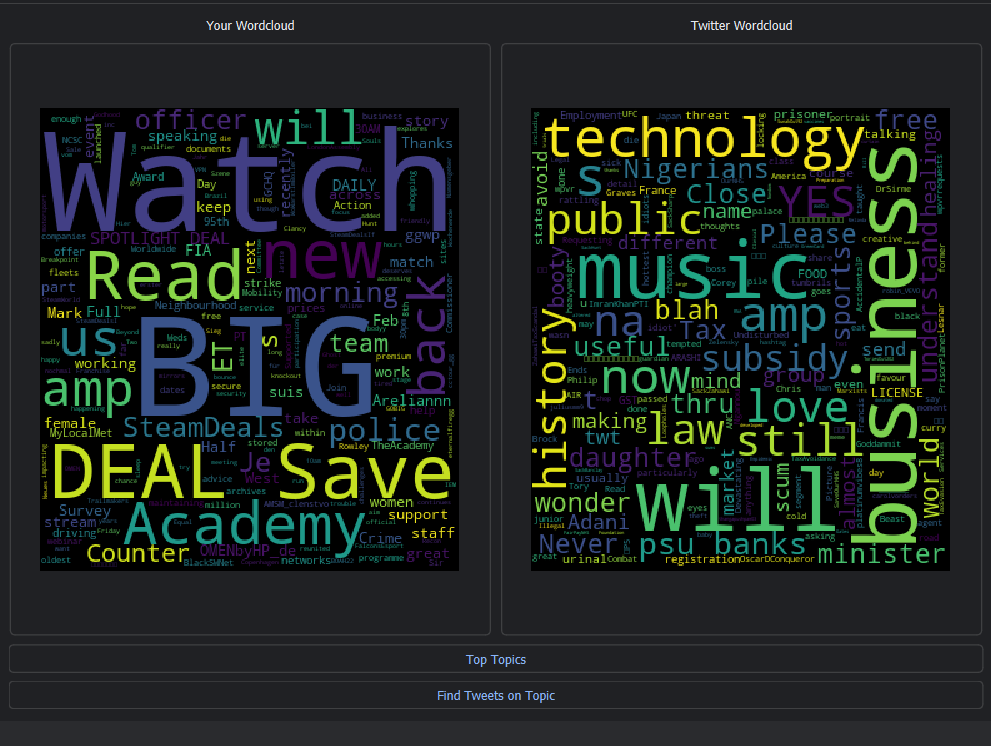
\includegraphics[width=0.8\textwidth]{../images/UI-dark-1-wc.png}
    \caption{Final UI design - Wordcloud}
    \label{fig:ui-wordcloud}
\end{figure}
\begin{figure}[h]
    \centering
    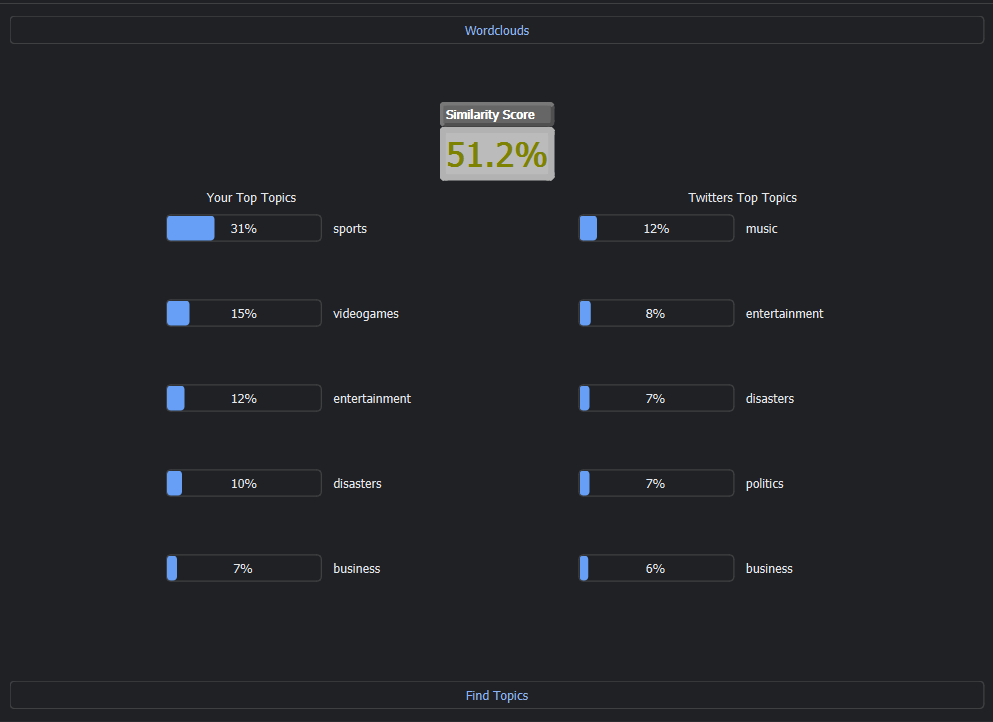
\includegraphics[width=0.8\textwidth]{../images/UI-dark-1-tt.png}
    \caption{Final UI design - Wordcloud}
    \label{fig:ui-toptopics}
\end{figure}
\begin{figure}[h]
    \centering
    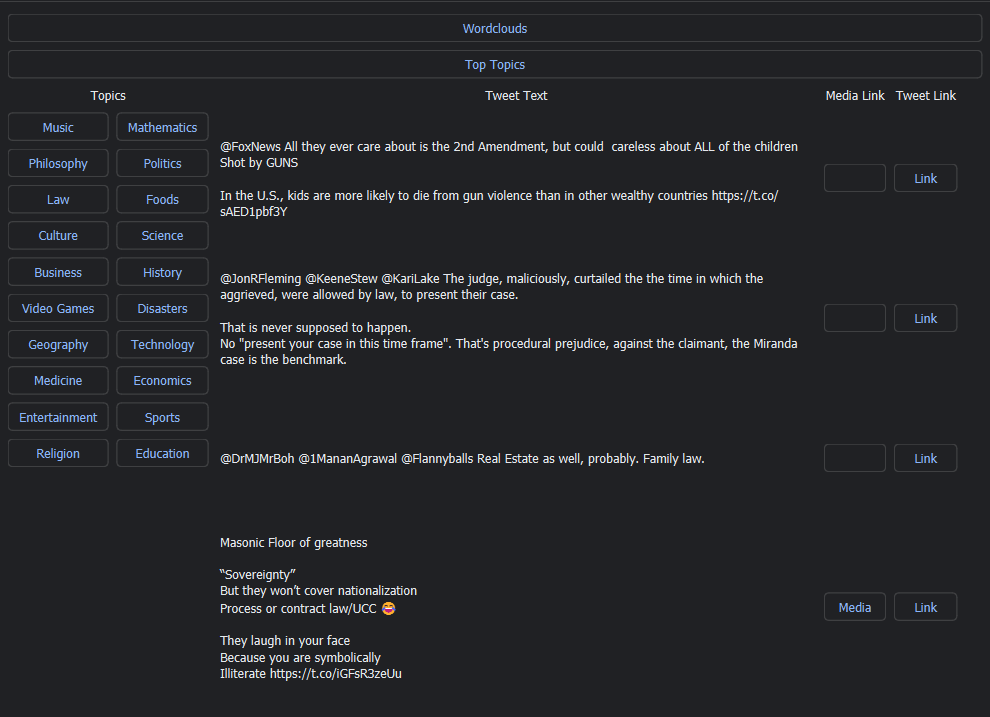
\includegraphics[width=0.8\textwidth]{../images/UI-dark-1-ft.png}
    \caption{Final UI design - Wordcloud}
    \label{fig:ui-findtopics}
\end{figure}

TODO: discuss pros and cons of design
Discuss PyQT and how it was used
Discuss benefits to PyQT designer
Discuss development of UI

\subsection{Backend}
The backend was also developed using Python. This allowed for easy integration with the frontend. In fact, the backend was developed as a standalone
class that could be imported into the frontend and used directly. The design shown in \cref{fig:backend} shows how the backend works. The design
ignores any implementation specific details. For example, the design just shows that there is tweets and not how the tweets are retrieved.
While working with the `tweepy' library, multiple methods for retrieving tweets were used. The first method was to use the `get\_home\_timeline'
method. This returns the most recent tweets from the user's home timeline. The second method was using a `StreamingClient' to listen for
live tweets. Finally, the use of the `get\_tweets' method was used to retrieve specific tweets via ID. On top of this, as discussed in \cref{sec:context_aware_model}
the use of the `conversation\_id' tweet\_field was used so that the retweets/replies to a tweet could be retrieved.
For retrieving live tweets check Appendix \ref{app:live-tweets} for the code used.\\
For retrieving users tweets check Appendix \ref{app:users-tweets} for the code used.\\\\
The backend databse schema laid out in \cref{ch:design} required slight adjustments to include the ability to store tweets with the same `conversation\_id'.
It also required the addition of a `hashtags' table to store the hashtags found in tweets sorted by topic.
This was overlooked originally as the design was based on the assumption of using the base RoBERTa model and not the context aware model.
Below is the updated schema
\begin{figure}[h]
    \centering
    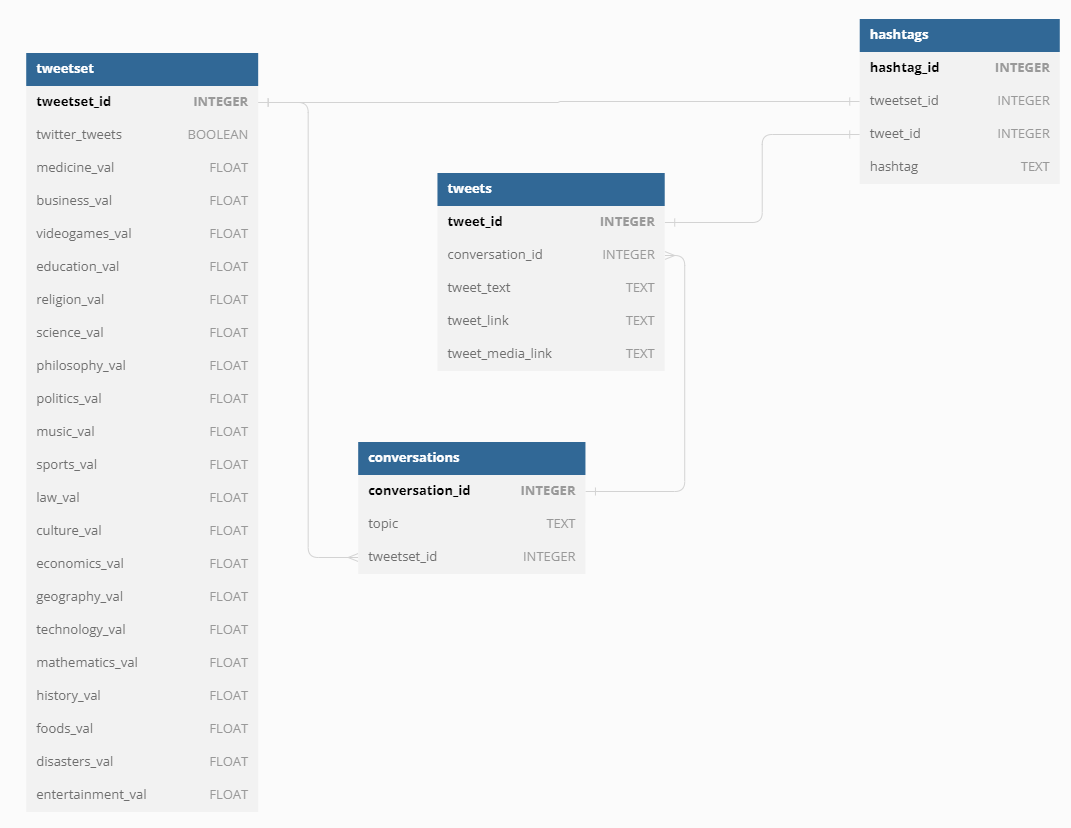
\includegraphics[width=0.8\textwidth]{../images/updated-schema.png}
    \caption{Updated database schema}
    \label{fig:updated-schema}
\end{figure}

The next step is to create the queries to create/update/retrieve data from the database in-line with the schema and backend design. Queries required:
\begin{enumerate}
    \item Create tweet
    \begin{algorithm}
        \begin{algorithmic}
            \STATE INSERT INTO tweets VALUES (NULL, conversation\_id, text, tweet\_url, media\_url)
        \end{algorithmic}
    \end{algorithm}
    \item Create conversation
    \begin{algorithm}
        \begin{algorithmic}
            \STATE INSERT INTO conversations VALUES (conversation\_id, NULL, tweetset\_id)
        \end{algorithmic}
    \end{algorithm}
    \item Create tweetset
    \begin{algorithm}
        \begin{algorithmic}
            \STATE INSERT INTO tweetset VALUES (NULL, is\_live, NULL ($\times 20$))
        \end{algorithmic}
    \end{algorithm}
    \item Set conversation topic
    \begin{algorithm}
        \begin{algorithmic}
            \STATE UPDATE conversations SET topic=topic WHERE conversation\_id=conversation\_id
        \end{algorithmic}
    \end{algorithm}
    \item Set tweetset topic scores
    \begin{algorithm}
        \begin{algorithmic}
            \STATE UPDATE tweetset SET medicine\_val=medicine\_val, ... WHERE tweetset\_id=tweetset\_id
        \end{algorithmic}
    \end{algorithm}
    \item Get hashtags for topic
    \begin{algorithm}
        \begin{algorithmic}
            \STATE SELECT hashtag FROM hashtags WHERE tweetset\_id=tweetset\_id AND tweet\_id IN (SELECT tweet\_id FROM tweets INNER JOIN conversations ON tweets.conversation\_id=conversations.conversation\_id WHERE conversation.topic=topic)
        \end{algorithmic}
    \end{algorithm}
    \item Get top topics for tweetset
    \begin{algorithm}
        \begin{algorithmic}
            \STATE SELECT * FROM tweetset WHERE tweetset\_id=tweetset\_id
        \end{algorithmic}
    \end{algorithm}
    \item Get tweets for a given tweetset
    \begin{algorithm}
        \begin{algorithmic}
            \STATE SELECT tweets.text, tweets.tweet\_url, tweets.media\_url, conversations.topic FROM tweets INNER JOIN conversations ON tweets.conversation\_id=conversations.conversation\_id WHERE conversations.tweetset\_id=tweetset\_id
        \end{algorithmic}
    \end{algorithm}
    \item Get tweets for a given topic
    \begin{algorithm}
        \begin{algorithmic}
            \STATE SELECT text, tweet\_url, media\_url FROM tweetset INNER JOIN conversations ON tweets.tweetset\_id=conversations.tweetset\_id INNER JOIN tweets ON conversations.conversation\_id=tweets.conversation\_id WHERE conversations.topic=topic
        \end{algorithmic}
    \end{algorithm}
\end{enumerate}
Discuss how the backend was created
Develop on database architecture to show how data is retrieved
Show SQL queries used
\section{Implementation Strategy}
\subsection{Model Creation}
While creating the different models for the topic detection an iterative approach was used. This allowed for the design, implementation and testing
of each model to be done in a short period of time and then move on to the next model. This waterfall-like approach works well for model creation,
especially with the RoBERTa model; the first iteration of the model created the base topic classification model. This model was then used
in the second iteration to create the context aware model.
Discuss iterative development cycle and how a waterfall sub approach was used
Explain why this approach worked well
backup with evidence
\subsection{Python Application}
For the Python application, an agile Kanban approach was used. This was partly due to the time constraints, but also because it allowed for
any minor changes required during development to be easily implemented. The Kanban board created consisted of the following columns:
\begin{itemize}
    \item Ideas
    \item Designs
    \item In-Progress
    \item Testing
    \item Completed
\end{itemize}
Due to the fact this project was a solo project, the need for a more complex Kanban board was not required. On top of this, the solo project
means less focus on how items move through the board is required. Usually, items would move using a given protocol (e.g. pull system). For this
project the Kanban board was treated as a simple to-do list and allowed a visual representation of the status of the project.
Discuss how an agile Kanban approach was used
explain why this approach worked well
backup with evidence